\chapter{Space-Based Architecture}
\label{bab:ruang}

\section*{Tujuan Pembelajaran}

\begin{enumerate}
  \item Menjelaskan bagian susunan berbasis \textit{tuple space} beserta
    peran ruang yang menggantikan basis data di jalur permintaan.
  \item Membedakan jalur data yang melewati basis data dari jalur data yang
    melewati memori, lalu menentukan kapan masing-masing layak dipilih.
  \item Mengukur \textit{throughput scaling}, \textit{stale read}, dan
    \textit{data loss} pada kedua versi.
\end{enumerate}

\section{Pendahuluan}

\textit{Space-based architecture} menjawab satu persoalan yang sempit, yaitu
titik sempit pada basis data. Sebuah aplikasi dapat disalin ke sepuluh mesin
tanpa kesulitan berarti. Basis datanya tidak. Ketika kesepuluh salinan itu
menulis ke satu \textit{file} yang sama, giliran menulis itulah yang menentukan hasil
akhirnya, bukan banyaknya mesin.

Jalan keluarnya membalik kebiasaan. Data yang dibutuhkan pada setiap permintaan
dipindahkan ke memori setiap \textit{processing unit}, lalu penyimpanan ke basis data
dikerjakan belakangan oleh bagian lain. \textit{Processing unit} tidak lagi menunggu
\textit{file}, sehingga menambah unit benar-benar menambah hasil. Nama susunannya
diambil dari ruang bersama tempat unit bertukar data, dan gagasan ruang itu
sendiri sudah berumur empat dekade~\cite{gelernter1985linda}.

Bab ini menyusun satu aplikasi pemroses setoran valuta asing dalam dua versi
dengan domain yang sama persis, lalu mengukur keduanya. Yang diukur bukan hanya
kecepatannya, melainkan juga harga yang dibayarnya, yaitu data basi dan data
yang lenyap. Pembahasan mengikuti kerangka yang disusun oleh Richards dan
Ford~\cite{richards2020fundamentals}.

\section{Bagian Susunan Berbasis \textit{Tuple Space}}

Susunannya dibagi menjadi tiga kelompok. \textbf{\textit{Processing unit}} memuat modul
aplikasi beserta salinan data yang dibutuhkannya di dalam memori.
\textbf{Middleware tervirtualisasi} mengurus segala hal di antara unit, yaitu
pembagian permintaan, replikasi data, dan penyalaan unit baru. \textbf{Pompa
data} beserta penulis dan pembacanya menghubungkan seluruhnya dengan basis data,
dan justru bagian inilah yang dijauhkan dari jalur permintaan.

Gambar~\ref{fig:topologi-ruang} menunjukkan susunannya. Perhatikan bahwa tidak
ada satu pun panah dari \textit{processing unit} yang langsung menuju basis data.

\begin{figure}[htbp]
  \centering
  \begin{tikzpicture}[
    kotak/.style={draw, rounded corners=2pt, align=center,
      font=\tiny\bfseries},
    unit/.style={kotak, fill=praditagreen!25, minimum width=3.2cm,
      minimum height=0.95cm},
    bagian/.style={kotak, fill=blue!8, minimum width=2.45cm,
      minimum height=0.8cm},
    simpan/.style={kotak, fill=green!10, minimum width=2.35cm,
      minimum height=0.75cm},
    panah/.style={-{Stealth[length=2mm]}, thick}
  ]
    \node[unit] (u1) {Processing unit 1\\
      {\tiny\mdseries modul + grid memori}};
    \node[unit, right=0.3cm of u1] (u2) {Processing unit 2\\
      {\tiny\mdseries modul + grid memori}};
    \node[unit, right=0.3cm of u2] (u3) {Processing unit 3\\
      {\tiny\mdseries modul + grid memori}};

    \node[bagian, below=1.25cm of u1] (pesan) {Messaging grid\\
      {\tiny\mdseries membagi permintaan}};
    \node[bagian, right=0.3cm of pesan] (data) {Data grid\\
      {\tiny\mdseries mereplikasi kurs}};
    \node[bagian, right=0.3cm of data] (kelola) {Deployment manager\\
      {\tiny\mdseries menyalakan unit}};

    \begin{scope}[on background layer]
      \node[draw, dashed, rounded corners=3pt, fill=praditagreen!8,
        inner ysep=11pt, inner xsep=5pt, fit=(pesan)(data)(kelola)] (mw) {};
    \end{scope}
    \node[font=\tiny\bfseries, anchor=north west]
      at ([shift={(0.12cm,-0.04cm)}]mw.north west) {Middleware tervirtualisasi};

    \node[simpan, below=1.25cm of data] (penulis) {Data writer\\
      {\tiny\mdseries commit sekelompok}};
    \node[simpan, left=0.7cm of penulis, fill=blue!8] (pembaca) {Data reader\\
      {\tiny\mdseries mengisi grid}};
    \node[kotak, fill=gray!22, right=0.7cm of penulis, minimum width=2.15cm,
      minimum height=0.75cm] (basis) {Basis data\\
      {\tiny\mdseries \textit{system of record}}};

    \draw[panah] (u1) -- (u1|-mw.north);
    \draw[panah] (u2) -- (u2|-mw.north);
    \draw[panah] (u3) -- (u3|-mw.north);
    \draw[panah] (data) -- node[right, font=\tiny\mdseries, pos=0.38]
      {data pump} (penulis);
    \draw[panah] (penulis) -- (basis);
    \draw[panah] (basis) |- ([yshift=-0.45cm]pembaca.south) -- (pembaca);
    \draw[panah] (pembaca) -- (pembaca|-mw.south);
  \end{tikzpicture}
  \caption{Susunan berbasis ruang. \textit{Processing unit} hanya berurusan dengan
    middleware, sedangkan basis data dijangkau lewat \textit{data pump} di luar jalur
    permintaan}
  \label{fig:topologi-ruang}
\end{figure}

Pembagian tersebut menentukan letak setiap keputusan.
Tabel~\ref{tab:bagian-ruang} merangkum tugas tiap bagian beserta wujudnya pada
kode bab ini. Dua bagian sengaja tidak dibuat, sebab keduanya baru masuk akal
bila unit tersebar di beberapa mesin.

\begin{table}[htbp]
  \centering
  \caption{Bagian susunan berbasis ruang beserta wujudnya pada kode bab ini}
  \label{tab:bagian-ruang}
  \begin{tabularx}{\textwidth}{|l|X|l|}
    \hline
    \textbf{Bagian} & \textbf{Tugasnya} & \textbf{Pada bab ini} \\
    \hline
    \textit{Processing unit} & Mengerjakan permintaan memakai data di memorinya sendiri & \texttt{UnitRuang} \\
    \hline
    \textit{Messaging grid} & Membagikan permintaan kepada unit yang sedang menganggur & \texttt{Ruang} \\
    \hline
    \textit{Data grid} & Menyimpan data bersama lalu mereplikasinya ke tiap unit & \texttt{Ruang} \\
    \hline
    \textit{Data pump} dan penulisnya & Memindahkan hasil ke basis data di luar jalur permintaan & \texttt{PenulisData} \\
    \hline
    \textit{Processing grid} & Memecah satu permintaan ke beberapa unit sekaligus & tidak dibuat \\
    \hline
    Deployment manager & Menyalakan dan mematikan unit mengikuti beban & tidak dibuat \\
    \hline
  \end{tabularx}
\end{table}

\section{\textit{Tuple Space} dan Tiga Operasinya}

Inti seluruh susunan itu satu benda saja, yaitu \textit{tuple space} atau ruang
tupel. Ruang adalah tempat menaruh data berbentuk tupel, dan pengambilannya
dilakukan dengan menyebutkan pola, bukan alamat. Gelernter menyebut cara
berkomunikasi seperti itu \textit{generative communication}, sebab tupel yang
sudah ditulis hidup sendiri di dalam ruang, terlepas dari nasib penulisnya,
sampai ada pihak lain yang mengambilnya~\cite{gelernter1985linda}.

Bahasa Linda menyediakan tiga operasi dasar, dan ketiganya diterjemahkan apa
adanya pada kode bab ini. Tabel~\ref{tab:operasi-linda} memasangkan keduanya.

\begin{table}[htbp]
  \centering
  \caption{Tiga operasi Linda beserta padanannya pada kelas \texttt{Ruang}}
  \label{tab:operasi-linda}
  \begin{tabularx}{\textwidth}{|l|l|X|}
    \hline
    \textbf{Linda} & \textbf{Kelas \texttt{Ruang}} & \textbf{Akibatnya pada isi ruang} \\
    \hline
    \texttt{out} & \texttt{tulis} & Tupel bertambah satu, dan penulisnya tidak menunggu siapa pun \\
    \hline
    \texttt{in} & \texttt{ambil} & Tupel yang cocok dikeluarkan, dan hanya satu pengambil yang mendapatkannya \\
    \hline
    \texttt{rd} & \texttt{baca} & Tupel yang cocok disalin, dan tupelnya tetap tinggal bagi pembaca lain \\
    \hline
  \end{tabularx}
\end{table}

Perbedaan antara \texttt{ambil} dan \texttt{baca} itulah yang membuat satu ruang
dapat memikul dua peran sekaligus. Tugas ditulis lalu diambil, sehingga satu
tugas dikerjakan tepat satu unit. Kurs ditulis lalu dibaca, sehingga seluruh
unit memperoleh kurs yang sama tanpa saling menunggu.

Padanan sehari-harinya papan pengumuman di lorong jurusan. Petugas menempel
selembar pengumuman lalu pergi, tanpa tahu siapa yang akan membacanya, dan
pengumuman itu tetap menempel walaupun petugasnya sudah pulang. Di sebelahnya
tergantung setumpuk formulir cuti. Pengumuman dibaca banyak orang dan tetap
tertempel, sedangkan formulir yang sudah diambil satu mahasiswa tidak mungkin
diambil mahasiswa berikutnya.

Listing~\ref{lst:ruang} memperlihatkan kedua operasi itu berdampingan. Keduanya
memanggil penolong yang sama, dan yang membedakannya hanya satu argumen.

\begin{lstlisting}[style=PythonStyle, caption={Dua operasi yang membedakan
  pengambilan dari pembacaan, tersedia di \berkas{sources/chapter08/ruang.py}},
  label=lst:ruang]
def ambil(self, pola: tuple, batas_waktu: float | None = None) -> tuple | None:
  """Mengeluarkan satu tupel yang memenuhi pola dari ruang."""
  return self._tunggu_cocok(pola, True, batas_waktu)

def baca(self, pola: tuple, batas_waktu: float | None = None) -> tuple | None:
  """Membaca satu tupel yang memenuhi pola tanpa mengeluarkannya."""
  return self._tunggu_cocok(pola, False, batas_waktu)
\end{lstlisting}

Sifat pengambilan tersebut dapat dibuktikan, bukan sekadar dijanjikan. \textit{File}
\texttt{ruang.py} menyalakan dua pengambil sekaligus atas satu tupel yang sama,
lalu melaporkan berapa pengambil yang berhasil. Jawabannya selalu satu dari dua,
sebab pencarian dan pengeluaran dikerjakan di bawah satu kunci yang sama.

\section{Satu Domain, Dua Jalur Data}

Kedua versi aplikasi pada bab ini memakai domain yang sama persis, yaitu satu
\textit{file} setoran berisi tiga ribu baris transaksi valuta asing yang dikonversi
lalu dijumlahkan. Nilai kursnya meniru kurs referensi Jakarta Interbank Spot
Dollar Rate (JISDOR) yang diterbitkan Bank Indonesia setiap hari kerja, yaitu
angka yang jarang berubah dalam sehari. Yang berbeda hanya tempat unit membaca
kurs dan tempat unit menaruh hasil.

Gambar~\ref{fig:kelas-ruang} menunjukkan perbedaan itu sebagai diagram kelas.
Arah panahnya yang layak diperhatikan, bukan jumlah kelasnya.

\begin{figure}[htbp]
  \centering
  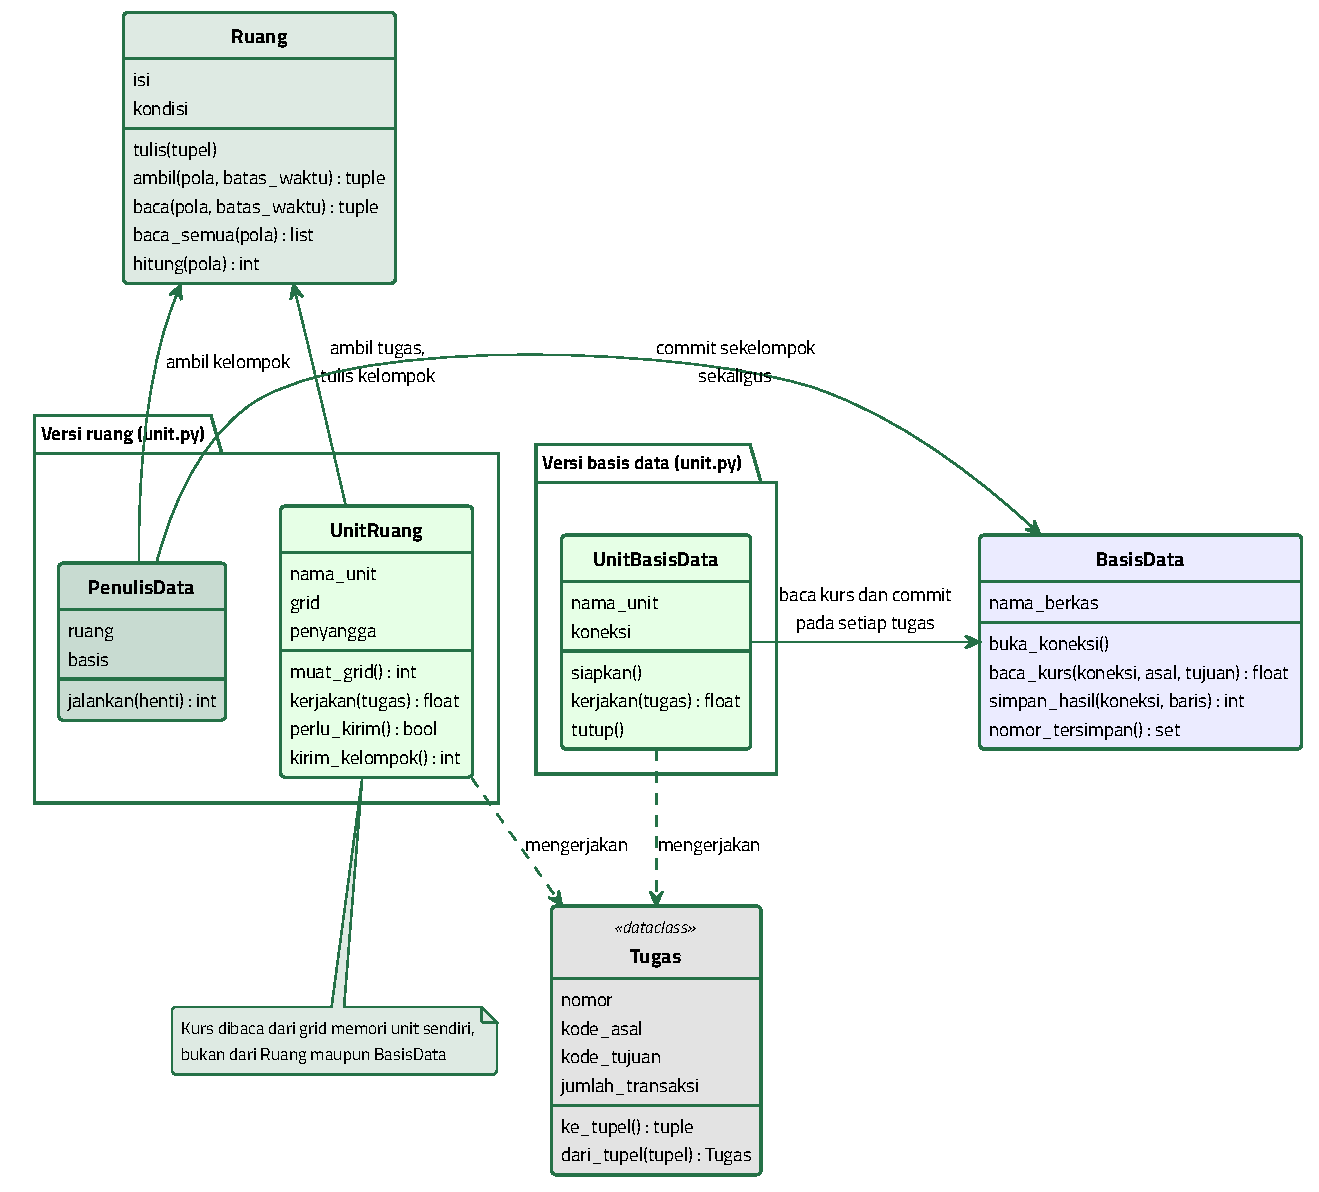
\includegraphics[width=\textwidth, height=0.42\textheight,
    keepaspectratio]{kelas-ruang.pdf}
  \caption{\texttt{UnitBasisData} menunjuk langsung ke \textit{file} SQLite, sedangkan
    \texttt{UnitRuang} hanya menunjuk ke ruang, dan \texttt{PenulisData} yang
    menyambungkannya dengan \textit{file}}
  \label{fig:kelas-ruang}
\end{figure}

Isi kedua unit pun hampir sama panjangnya. Listing~\ref{lst:unit-basis}
memperlihatkan versi basis data. Ketiga langkahnya, yaitu membaca kurs,
menghitung, dan menyimpan, seluruhnya berada di jalur setiap tugas.

\begin{lstlisting}[style=PythonStyle, caption={Satu tugas pada versi basis data,
  tersedia di \berkas{sources/chapter08/unit.py}}, label=lst:unit-basis]
def kerjakan(self, tugas: domain.Tugas) -> float:
  """Membaca kurs, menghitung total, lalu menyimpan hasilnya dalam satu commit."""
  mulai = time.perf_counter()
  kurs = self.basis.baca_kurs(self.koneksi, tugas.kode_asal, tugas.kode_tujuan)
  total = domain.hitung_total(tugas, kurs)
  self.basis.simpan_hasil(self.koneksi, [(tugas.nomor, self.nama_unit, total)])
  return (time.perf_counter() - mulai) * 1000.0
\end{lstlisting}

Versi ruang mengerjakan perhitungan yang sama persis, tetapi tidak menyentuh
\textit{file} sama sekali. Kurs diambil dari \texttt{self.grid}, yaitu salinan yang
sudah ada di memori unit, dan hasilnya ditumpuk di \texttt{self.penyangga}.
Listing~\ref{lst:unit-ruang} memperlihatkannya.

\begin{lstlisting}[style=PythonStyle, caption={Satu tugas pada versi ruang,
  tersedia di \berkas{sources/chapter08/unit.py}}, label=lst:unit-ruang]
def kerjakan(self, tugas: domain.Tugas) -> float:
  """Menghitung total tugas memakai kurs lokal, lalu menumpuk hasilnya."""
  mulai = time.perf_counter()
  kurs = self.grid.get((tugas.kode_asal, tugas.kode_tujuan))
  total = domain.hitung_total(tugas, kurs)
  self.penyangga.append((tugas.nomor, self.nama_unit, total))
  if self.perlu_kirim():
    self.kirim_kelompok()
  return (time.perf_counter() - mulai) * 1000.0
\end{lstlisting}

Penyangga itu dikirim ke ruang hanya bila sudah berisi lima puluh hasil atau
sudah tertahan lebih dari 0,25 detik. Cara tersebut bukan karangan bab ini.
Apache Ignite menyebutnya \textit{write-behind}, yaitu perubahan dikumpulkan
lalu dikirim ke penyimpanan sebagai satu operasi kelompok, dan pengirimannya
dipicu oleh batas waktu, batas panjang antrean, atau keduanya
sekaligus~\cite{ignite2026docs}.

Gambar~\ref{fig:sekuens-ruang} menyandingkan satu tugas yang sama pada kedua
versi. Perbedaannya bukan pada perhitungannya, melainkan pada apa yang ditunggu
sesudahnya.

\begin{figure}[htbp]
  \centering
  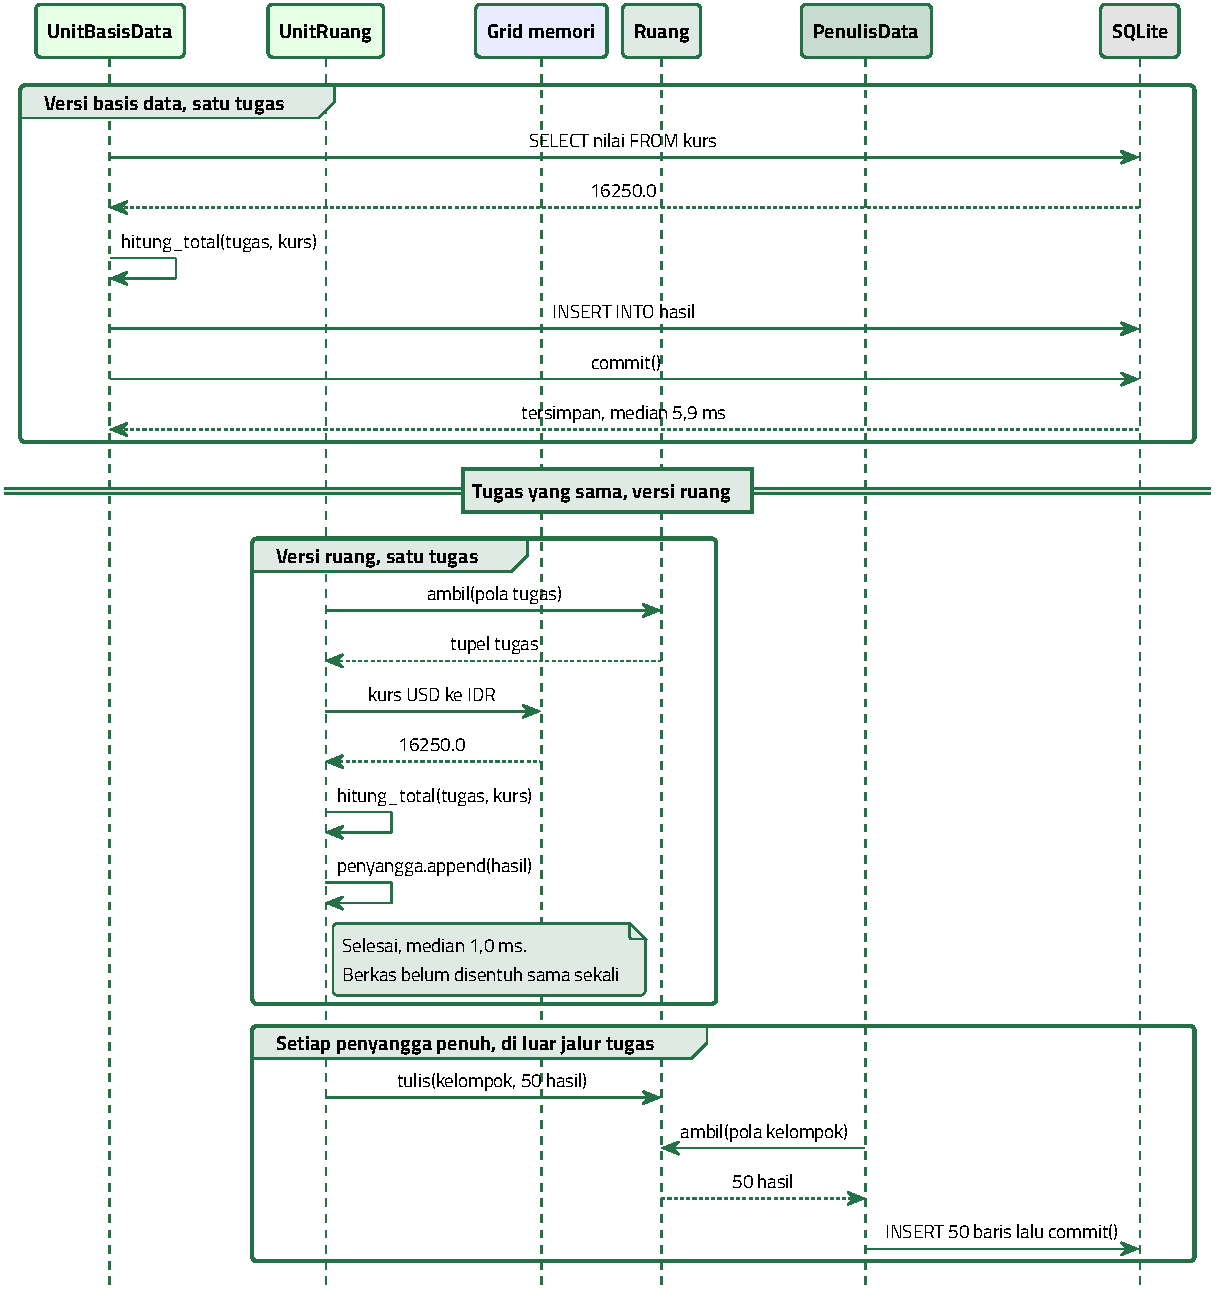
\includegraphics[width=\textwidth, height=0.52\textheight,
    keepaspectratio]{sekuens-ruang.pdf}
  \caption{Satu tugas yang sama pada kedua versi. Versi basis data menunggu
    commit selesai, sedangkan versi ruang selesai begitu hasilnya masuk
    penyangga}
  \label{fig:sekuens-ruang}
\end{figure}

Perbedaan itu punya dua akibat yang berlawanan arah. Pertama, tugas pada versi
ruang selesai jauh lebih cepat, sebab tidak ada yang ditunggu. Kedua, tugas yang
sudah dinyatakan selesai itu belum tersimpan di mana pun kecuali di memori satu
unit. Akibat pertama diukur pada seksi berikutnya, sedangkan akibat kedua diukur
pada seksi terakhir.

\section{Menambah \textit{Processing Unit}}

Pertanyaan yang paling langsung adalah apakah menambah \textit{processing unit} memang
menambah hasil. Beban yang dipakai tetap, yaitu 900 tugas berisi tiga ribu
transaksi masing-masing, dan jumlah unitnya dinaikkan dari satu menjadi delapan.
Setiap susunan diulang lima putaran, dan urutannya berselang-seling agar
kesibukan sesaat di luar percobaan tidak menimpa satu susunan saja.

Perbandingannya sengaja dibuat berpihak kepada versi basis data. Koneksi SQLite
dibuka sekali lalu dipakai ulang, sehingga biaya membuka \textit{file} tidak terhitung
pada setiap tugas. Tugasnya pun dibagikan lewat pencacah bersama yang murah,
sedangkan versi ruang harus mengambil tugasnya lewat soket. Selisih yang terukur
karena itu adalah batas bawahnya.

Tabel~\ref{tab:hasil-unit} memuat hasilnya apa adanya. Pengukurannya dijalankan
pada laptop berprosesor empat inti dengan delapan utas.

\begin{table}[htbp]
  \centering
  \small
  \caption{\textit{Throughput} dan sebaran latensi kedua versi, lima putaran
    tiap susunan}
  \label{tab:hasil-unit}
  \begin{tabularx}{\textwidth}{|l|X|r|r|r|r|}
    \hline
    \textbf{Unit} & \textbf{Versi} & \textbf{Tugas/detik} & \textbf{Median ms} & \textbf{Persentil ke-95 ms} & \textbf{Terbesar ms} \\
    \hline
    1 & basis data & 319,1 & 3,118 & 4,019 & 24,359 \\
    \hline
    2 & basis data & 298,6 & 3,229 & 9,427 & 1437,879 \\
    \hline
    4 & basis data & 244,3 & 4,153 & 57,045 & 1835,463 \\
    \hline
    8 & basis data & 273,0 & 4,250 & 109,292 & 1936,111 \\
    \hline
    1 & ruang & 1307,7 & 0,625 & 1,011 & 2,026 \\
    \hline
    2 & ruang & 2457,1 & 0,596 & 1,264 & 3,913 \\
    \hline
    4 & ruang & 3594,1 & 0,719 & 1,765 & 3,817 \\
    \hline
    8 & ruang & 4007,5 & 1,480 & 2,683 & 6,588 \\
    \hline
  \end{tabularx}
\end{table}

Tiga hal layak dibaca dari tabel tersebut. Pertama, versi basis data tidak
bertambah hasilnya ketika unitnya ditambah. Angkanya justru turun dari 319,1
tugas per detik pada satu unit menjadi 244,3 pada empat unit, lalu naik sedikit
menjadi 273,0 pada delapan unit. Menambah unit hanya menambah pengantre pada
\textit{file} yang sama.

Kedua, versi ruang bertambah hasilnya, tetapi tidak sebanding jumlah unitnya.
Dari satu unit ke dua unit, hasilnya naik 1,9 kali. Dari satu unit ke empat
unit, naik 2,7 kali. Dari satu unit ke delapan unit, hanya naik 3,1 kali.
Laptop percobaannya berinti empat, sehingga unit kelima sampai kedelapan
berebut inti yang sama.

Ketiga, selisih keduanya melebar mengikuti jumlah unit, yaitu 4,1 kali pada satu
unit, lalu 14,7 kali pada empat maupun delapan unit. Selisih itulah batas
bawahnya, sebab percobaannya sengaja dibuat berpihak kepada versi basis data.

Kolom latensi memuat gejala yang tidak tampak pada kolom hasil. Median versi
basis data hanya naik dari 3,118 ms menjadi 4,250 ms, seakan-akan beban
tambahannya ringan. Nilai terbesarnya bercerita lain, yaitu melonjak dari 24,359
ms menjadi 1936,111 ms. Lonjakan pada nilai terbesar itulah tanda antrean, dan
median menyembunyikannya. Pada versi ruang, nilai terbesarnya tetap di bawah
tujuh milidetik walaupun unitnya delapan.

\section{Replikasi yang Tertunda}

Kecepatan tersebut ditebus dengan sesuatu. Tebusan yang pertama adalah kurs yang
sudah tidak berlaku lagi. Unit membaca kurs dari grid memorinya sendiri, dan
grid itu hanya disegarkan berkala. Selama jeda penyegaran, unit tetap bekerja
memakai kurs lama walaupun kurs baru sudah terbit. Pembacaan seperti itu disebut
\textit{stale read}, dan Richards serta Ford menyebut akibat buruknya \textit{data
collision}~\cite{richards2020fundamentals}.

Banyaknya \textit{stale read} dapat dihitung, bukan sekadar dikhawatirkan. Skrip
\texttt{ukur\_basi.py} menerbitkan kurs baru setiap 50 milidetik, lalu
menjalankan empat pembaca yang menyegarkan gridnya pada beberapa jeda yang
berbeda. Setiap jeda dicoba tiga putaran satu detik.
Tabel~\ref{tab:basi} memuat hasilnya.

\begin{table}[htbp]
  \centering
  \caption{\textit{Stale read} pada beberapa \textit{replication lag}, tiga
    putaran satu detik tiap jeda}
  \label{tab:basi}
  \begin{tabularx}{\textwidth}{|r|r|r|X|}
    \hline
    \textbf{\textit{Replication lag} (ms)} & \textbf{Pembacaan} & \textbf{\textit{Stale read}} & \textbf{Bagian basi} \\
    \hline
    0 & 11.048 & 0 & 0,0\% \\
    \hline
    5 & 11.063 & 439 & 4,0\% \\
    \hline
    10 & 11.029 & 1.034 & 9,4\% \\
    \hline
    25 & 11.046 & 2.519 & 22,8\% \\
    \hline
    50 & 11.067 & 1.052 & 9,5\% \\
    \hline
    100 & 11.055 & 5.937 & 53,7\% \\
    \hline
    200 & 11.056 & 8.564 & 77,5\% \\
    \hline
  \end{tabularx}
\end{table}

Jumlah pembacaannya hampir sama pada setiap baris, yaitu sekitar sebelas ribu,
sehingga selisih kolom terakhir benar-benar berasal dari jedanya. Tanpa jeda,
tidak satu pun \textit{stale read}, sebab grid disegarkan sebelum setiap pembacaan.
Jeda 200 ms membuat lebih dari tiga perempat pembacaannya basi, padahal jeda itu
masih terdengar singkat bagi manusia.

Satu baris menyimpang dari pola tersebut dan sebabnya perlu disebut. Jeda 50 ms
menghasilkan 9,5 persen \textit{stale read}, lebih kecil daripada jeda 25 ms yang
menghasilkan 22,8 persen. Sebabnya jeda itu sama persis dengan jarak terbitnya
kurs, yaitu 50 ms, sehingga penyegaran dan penerbitan berjalan pada denyut yang
sama lalu tetap sejalan sepanjang satu putaran. Penyegaran selalu tiba sesaat
sesudah kurs baru terbit, dan kurs lama hanya sempat terbaca pada celah yang
sempit.

Akibat \textit{stale read} tidak selalu sekecil selisih kurs. Sebuah kampus memakai
susunan berbasis ruang untuk sistem pengisian rencana studi. Sisa kuota setiap
kelas disalin ke grid memori tiap unit, dan replikasinya dijadwalkan setiap
dua ratus milidetik. Pada menit pertama pembukaan, ribuan mahasiswa menekan
tombol yang sama. Belasan unit membaca sisa kuota yang sama dari grid
masing-masing, lalu sama-sama menyimpulkan kursinya masih ada. Kelas berkuota
empat puluh terisi lima puluh tiga mahasiswa, dan tiga belas di antaranya
terpaksa dikeluarkan keesokan harinya.

\section{Harga yang Dibayar}

Tebusan yang kedua jauh lebih berat, yaitu data yang lenyap. Hasil yang masih
menumpuk di penyangga sebuah unit tidak berada di mana pun selain memori unit
itu. Bila unitnya mati sebelum penyangga terkirim, hasil itu hilang tanpa jejak,
dan tugasnya pun tidak mungkin diulang sebab tupelnya sudah terlanjur diambil
dari ruang.

Padanan sehari-harinya kasir warung yang mencatat penjualan pada secarik kertas,
lalu memindahkannya ke buku besar sekali saja menjelang tutup. Cara itu membuat
setiap pembeli dilayani cepat, sebab tidak ada yang menunggu buku besar dibuka.
Akan tetapi bila kertasnya hilang sebelum sempat dipindahkan, penjualan sesore
itu tidak berbekas di buku mana pun.

Apache Ignite mencantumkan peringatan yang sama persis pada dokumentasinya. Cara
\textit{write-behind} memang menaikkan hasil, akan tetapi konsistensinya dapat
menurun sebab sebagian perubahan dapat hilang ketika sebuah simpul gagal atau
mati mendadak~\cite{ignite2026docs}.

Skrip \texttt{uji\_kehilangan.py} mengukur kehilangan itu. Empat unit
mengerjakan 600 tugas, lalu satu unit dimatikan dengan SIGKILL tepat ketika
separuh beban sudah dibagikan. Sesudah unit yang tersisa menghabiskan sisanya,
baris pada tabel hasil dihitung lalu dibandingkan dengan 600.
Tabel~\ref{tab:kehilangan} memuat hasil lima putaran.

\begin{table}[htbp]
  \centering
  \caption{Tugas yang lenyap ketika satu unit dimatikan pada separuh beban}
  \label{tab:kehilangan}
  \begin{tabularx}{\textwidth}{|l|X|X|}
    \hline
    \textbf{Putaran} & \textbf{Hilang, versi basis data} & \textbf{Hilang, versi ruang} \\
    \hline
    1 & 1 tugas & 18 tugas \\
    \hline
    2 & 1 tugas & 28 tugas \\
    \hline
    3 & 1 tugas & 15 tugas \\
    \hline
    4 & 1 tugas & 35 tugas \\
    \hline
    5 & 1 tugas & 41 tugas \\
    \hline
    Median & 1 tugas & 28 tugas \\
    \hline
    \textit{Range} & 1 sampai 1 tugas & 15 sampai 41 tugas \\
    \hline
  \end{tabularx}
\end{table}

Versi basis data kehilangan tepat satu tugas pada kelima putaran, yaitu tugas
yang sedang dikerjakan ketika unitnya dimatikan. Hasil tugas sebelumnya sudah
masuk \textit{file}, sebab setiap tugas menuntaskan \textit{commit}-nya sendiri sebelum
dinyatakan selesai.

Versi ruang kehilangan 15 sampai 41 tugas, dengan median 28 tugas. Angka median
itu setara 84.000 transaksi yang sudah dihitung lalu lenyap tanpa jejak. Yang
hilang adalah isi penyangga unit tersebut, dan jumlahnya bergantung pada seberapa
penuh penyangga itu saat unitnya mati. Penyangga berisi paling banyak lima puluh
hasil, sehingga 41 tugas berarti unitnya mati ketika penyangganya hampir penuh.

Dua angka tersebut layak dibaca berdampingan dengan tabel sebelumnya. Versi
ruang 14,7 kali lebih cepat pada empat unit, dan harga yang dibayarnya 28 kali
lebih banyak tugas yang lenyap ketika satu unit mati. Keduanya datang dari
keputusan yang sama, yaitu memindahkan penyimpanan ke luar jalur permintaan.

Besar kehilangan itu bukan sifat bawaan susunannya, melainkan akibat satu
angka yang dapat diubah, yaitu ukuran kelompok pada penyangga. Dengan ukuran
kelompok satu, yaitu setiap hasil langsung dikirim ke ruang, kehilangannya turun
menjadi satu tugas pada kelima putaran, sama dengan versi basis data. Hasil per
detiknya pada empat unit tercatat 3366,2 tugas per detik, sedangkan dengan
ukuran kelompok lima puluh tercatat 3594,1 pada percobaan sebelumnya. Harga
keamanan itu karena itu sekitar enam persen hasil pada mesin percobaan ini, dan
Latihan~3 meminta angkanya diukur ulang di mesin sendiri.

\section{Ringkasan}

\textit{Space-based architecture} lahir dari satu titik sempit yang nyata, yaitu
\textit{file} basis data yang dipakai bersama. Aplikasinya dapat disalin ke berapa pun
mesin, sedangkan berkasnya tidak, sehingga giliran menulislah yang menentukan
hasil akhir. Jalan keluarnya memindahkan data yang dibutuhkan setiap permintaan
ke memori tiap unit, lalu menaruh penyimpanan ke basis data di luar jalur
permintaan.

Inti susunannya satu benda, yaitu \textit{tuple space} beserta tiga operasinya. Tupel
yang ditulis hidup sendiri di dalam ruang, terlepas dari nasib penulisnya.
Pengambilan mengeluarkan tupelnya sehingga satu tugas dikerjakan tepat satu
unit, sedangkan pembacaan menyalinnya sehingga seluruh unit memperoleh kurs yang
sama tanpa saling menunggu. Perbedaan dua operasi itulah yang membuat satu ruang
dapat memikul peran pembagi tugas sekaligus peran penyedia data.

Pengukurannya menjawab pertanyaan yang paling langsung. Versi basis data tidak
bertambah hasilnya ketika unitnya ditambah, yaitu 319,1 tugas per detik pada satu
unit dan 244,3 pada empat unit. Versi ruang naik dari 1307,7 menjadi 3594,1 pada
jumlah unit yang sama, sehingga selisihnya melebar menjadi 14,7 kali. Nilai
terbesar latensinya memperlihatkan sebabnya, yaitu 1936,111 ms pada versi basis
data melawan 3,817 ms pada versi ruang.

Kecepatan itu ditebus dua kali. Tebusan pertama kurs yang sudah tidak berlaku,
dan besarnya mengikuti \textit{replication lag}, yaitu 4,0 persen \textit{stale read} pada jeda
5 ms sampai 77,5 persen pada jeda 200 ms. Tebusan kedua lebih berat, yaitu hasil
yang lenyap bersama unit yang mati. Versi basis data kehilangan satu tugas,
sedangkan versi ruang kehilangan 28 tugas atau 84.000 transaksi.

Pesan utama bab ini karena itu bukan bahwa ruang lebih cepat daripada basis
data. Keduanya menjawab pertanyaan yang berbeda. Ruang memindahkan penyimpanan
ke luar jalur permintaan, dan pemindahan itu membeli hasil per detik dengan
membayar ketepatan data pada saat yang paling buruk, yaitu ketika sebuah unit
mati.

\section{Latihan}

Ketiga latihan berikut memakai satu basis kode yang sama di
\berkas{sources/chapter08/}, tetapi menyasar tiga masalah yang berbeda.
Latihan~1 mengukur \textit{throughput scaling}. Latihan~2 mengukur
\textit{stale read}. Latihan~3 mengukur \textit{data loss}. Hasil setiap
mahasiswa akan berbeda mengikuti jumlah inti mesinnya, dan yang dilaporkan
adalah pola perbandingannya, bukan angka persisnya.

Penyiapannya dijalankan sekali seperti pada Listing~\ref{lst:venv-ch08}. Bab ini
hanya memakai pustaka standar Python, sehingga tidak ada pemasangan tambahan.

\begin{lstlisting}[language=bash, caption={Menyiapkan venv sebelum ketiga
  latihan, seluruh skrip tersedia di \berkas{sources/chapter08/}},
  label=lst:venv-ch08]
bash sources/siapkan_venv.sh
source .venv/bin/activate
cd sources/chapter08
python unit.py ruang 4
# Keluarannya: Versi              : ruang
#              Processing unit    : 4
#              Tugas per detik    : 3815.9
#              Tugas tersimpan    : 900
\end{lstlisting}

\subsection*{Latihan 1: \textit{Throughput Scaling}}

Latihan ini menguji klaim utama susunan berbasis ruang, yaitu menambah unit
pemrosesan benar-benar menambah hasil. Klaim itu gugur bila hasil per detiknya
tidak naik walaupun unitnya digandakan. Langkah kerjanya sebagai berikut.

\begin{enumerate}
  \item Jalankan perintah pada Listing~\ref{lst:jalankan-hasil}, lalu catat
    kolom tugas per detik untuk kedelapan baris.
  \item Catat pula kolom median dan kolom terbesar, sebab keduanya menunjuk
    gejala yang berbeda.
  \item Hitung perbandingan hasil versi ruang terhadap versi basis data pada
    tiap jumlah unit, lalu bandingkan dengan jumlah inti mesin sendiri.
  \item Buka \berkas{sources/chapter08/ukur\_hasil.py}, ubah
    \texttt{JUMLAH\_UNIT} menjadi \texttt{(1, 2, 4, 8, 16)}, jalankan ulang,
    lalu catat apakah hasilnya masih naik pada 16 unit. Kembalikan nilainya
    sesudah dicatat.
\end{enumerate}

\begin{lstlisting}[language=bash, caption={Mengukur \textit{throughput
  scaling}, skrip tersedia di \berkas{sources/chapter08/ukur_hasil.py}},
  label=lst:jalankan-hasil]
python ukur_hasil.py
# Keluarannya: 1 basis data  319.1 tugas/detik  median 3.118 ms
#              4 basis data  244.3 tugas/detik  median 4.153 ms
#              1 ruang      1307.7 tugas/detik  median 0.625 ms
#              4 ruang      3594.1 tugas/detik  median 0.719 ms
#              Ruang berbanding basis data pada 4 unit : 14.7 kali
\end{lstlisting}

Tabel~\ref{tab:lat1ruang-contoh} berisi hasil satu kali pengukuran nyata pada
laptop berinti empat.

\begin{table}[htbp]
  \centering
  \caption{Contoh hasil Latihan 1 yang sudah terisi}
  \label{tab:lat1ruang-contoh}
  \begin{tabularx}{\textwidth}{|l|X|X|l|}
    \hline
    \textbf{Unit} & \textbf{Basis data, tugas/detik} & \textbf{Ruang, tugas/detik} & \textbf{Perbandingan} \\
    \hline
    1 & 319,1 & 1307,7 & 4,1 kali \\
    \hline
    2 & 298,6 & 2457,1 & 8,2 kali \\
    \hline
    4 & 244,3 & 3594,1 & 14,7 kali \\
    \hline
    8 & 273,0 & 4007,5 & 14,7 kali \\
    \hline
  \end{tabularx}
\end{table}

Isikan hasil pengukuran pada Tabel~\ref{tab:lat1ruang-hasil}.

\begin{table}[htbp]
  \centering
  \caption{Lembar isian Latihan 1}
  \label{tab:lat1ruang-hasil}
  \begin{tabularx}{\textwidth}{|l|X|X|l|}
    \hline
    \textbf{Unit} & \textbf{Basis data, tugas/detik} & \textbf{Ruang, tugas/detik} & \textbf{Perbandingan} \\
    \hline
    1 & \dots & \dots & \dots \\
    \hline
    2 & \dots & \dots & \dots \\
    \hline
    4 & \dots & \dots & \dots \\
    \hline
    8 & \dots & \dots & \dots \\
    \hline
    16 & \dots & \dots & \dots \\
    \hline
  \end{tabularx}
\end{table}

Jawab tiga pertanyaan berikut dengan menunjuk angka pada tabel. Pertama,
jelaskan mengapa hasil versi basis data tidak naik walaupun unitnya ditambah.
Kedua, sebutkan pada jumlah unit berapa hasil versi ruang berhenti naik di mesin
sendiri, lalu hubungkan angka itu dengan jumlah intinya. Ketiga, jelaskan
mengapa median latensi versi basis data hampir tidak berubah sedangkan nilai
terbesarnya melonjak.

\subsection*{Latihan 2: \textit{Stale Read}}

Latihan ini membuktikan bahwa kecepatan versi ruang ditebus dengan ketepatan
data. Kurs dibaca dari grid memori, dan grid itu hanya disegarkan berkala,
sehingga selama jedanya unit bekerja memakai kurs lama. Langkah kerjanya sebagai
berikut.

\begin{enumerate}
  \item Jalankan perintah pada Listing~\ref{lst:jalankan-basi}, lalu catat
    ketiga kolom untuk ketujuh jeda.
  \item Perhatikan baris jeda 50 ms, lalu jelaskan mengapa bagian basinya lebih
    kecil daripada baris jeda 25 ms.
  \item Buka \berkas{sources/chapter08/ukur\_basi.py}, ubah
    \texttt{JEDA\_PEMBARUAN} dari 0,05 menjadi 0,02 detik, jalankan ulang, lalu
    catat perubahan bagian basinya. Kembalikan nilainya sesudah dicatat.
\end{enumerate}

\begin{lstlisting}[language=bash, caption={Mengukur \textit{stale read}, skrip
  tersedia di \berkas{sources/chapter08/ukur_basi.py}}, label=lst:jalankan-basi]
python ukur_basi.py
# Keluarannya:   0 ms  11048 pembacaan      0 basi   0.0%
#                25 ms  11046 pembacaan   2519 basi  22.8%
#               200 ms  11056 pembacaan   8564 basi  77.5%
\end{lstlisting}

Tabel~\ref{tab:lat2ruang-contoh} berisi hasil satu kali pengukuran nyata.

\begin{table}[htbp]
  \centering
  \caption{Contoh hasil Latihan 2 yang sudah terisi}
  \label{tab:lat2ruang-contoh}
  \begin{tabularx}{\textwidth}{|r|r|r|X|}
    \hline
    \textbf{Jeda (ms)} & \textbf{Pembacaan} & \textbf{Basi} & \textbf{Bagian basi} \\
    \hline
    0 & 11.048 & 0 & 0,0\% \\
    \hline
    10 & 11.029 & 1.034 & 9,4\% \\
    \hline
    25 & 11.046 & 2.519 & 22,8\% \\
    \hline
    100 & 11.055 & 5.937 & 53,7\% \\
    \hline
    200 & 11.056 & 8.564 & 77,5\% \\
    \hline
  \end{tabularx}
\end{table}

Isikan hasil pengukuran pada Tabel~\ref{tab:lat2ruang-hasil}.

\begin{table}[htbp]
  \centering
  \caption{Lembar isian Latihan 2}
  \label{tab:lat2ruang-hasil}
  \begin{tabularx}{\textwidth}{|r|X|X|}
    \hline
    \textbf{Jeda (ms)} & \textbf{Bagian basi, kurs tiap 50 ms} & \textbf{Bagian basi, kurs tiap 20 ms} \\
    \hline
    0 & \dots & \dots \\
    \hline
    25 & \dots & \dots \\
    \hline
    100 & \dots & \dots \\
    \hline
    200 & \dots & \dots \\
    \hline
  \end{tabularx}
\end{table}

Jawab tiga pertanyaan berikut. Pertama, jelaskan mengapa jeda nol menghasilkan
nol \textit{stale read}, lalu sebutkan harga yang dibayar bila jeda itu benar-benar
dipakai. Kedua, jelaskan mengapa mempercepat terbitnya kurs menaikkan bagian
basi pada jeda yang sama. Ketiga, dengan memakai kasus pengisian rencana studi
pada bab ini, tentukan \textit{replication lag} yang masih dapat diterima beserta
alasannya.

\subsection*{Latihan 3: \textit{Data Loss}}

Latihan ini mengukur tebusan yang paling berat, yaitu hasil yang lenyap bersama
unit yang mati. Hasil yang masih menumpuk di penyangga belum berada di mana pun
selain memori unit itu. Langkah kerjanya sebagai berikut.

\begin{enumerate}
  \item Jalankan perintah pada Listing~\ref{lst:jalankan-hilang}, lalu catat
    kedua kolom untuk kelima putaran beserta median dan \textit{range}-nya.
  \item Buka \berkas{sources/chapter08/unit.py}, lalu tunjukkan baris yang
    menentukan kapan penyangga dikirim.
  \item Ubah \texttt{UKURAN\_KELOMPOK} dari 50 menjadi 1, jalankan ulang
    \texttt{python uji\_kehilangan.py}, lalu catat tugas yang hilang.
  \item Jalankan \texttt{python ukur\_hasil.py} dengan ukuran kelompok satu itu,
    lalu catat hasil per detiknya pada empat unit. Kembalikan nilainya sesudah
    dicatat.
\end{enumerate}

\begin{lstlisting}[language=bash, caption={Mengukur \textit{data loss}, skrip
  tersedia di \berkas{sources/chapter08/uji_kehilangan.py}},
  label=lst:jalankan-hilang]
python uji_kehilangan.py
# Keluarannya: Median tugas hilang, versi basis data : 1 tugas
#              Median tugas hilang, versi ruang      : 28 tugas
#              Range tugas hilang, versi ruang       : 15 sampai 41 tugas
\end{lstlisting}

Tabel~\ref{tab:lat3ruang-contoh} berisi hasil satu kali percobaan nyata.

\begin{table}[htbp]
  \centering
  \caption{Contoh hasil Latihan 3 yang sudah terisi, lima putaran}
  \label{tab:lat3ruang-contoh}
  \begin{tabularx}{\textwidth}{|X|l|l|}
    \hline
    \textbf{Yang dilaporkan} & \textbf{Basis data} & \textbf{Ruang} \\
    \hline
    Median tugas hilang & 1 & 28 \\
    \hline
    \textit{Range} tugas hilang & 1 sampai 1 & 15 sampai 41 \\
    \hline
    Transaksi hilang pada median & 3.000 & 84.000 \\
    \hline
    Median hilang, kelompok satu & 1 & 1 \\
    \hline
    Tugas per detik pada empat unit & 244,3 & 3366,2 \\
    \hline
  \end{tabularx}
\end{table}

Baris dua terakhir memuat percobaan dengan ukuran kelompok satu. Angka tugas per
detik versi ruang itu diambil dari penjalanan yang sama, sehingga dapat
dibandingkan dengan 3594,1 pada ukuran kelompok lima puluh.

Isikan hasil percobaan pada Tabel~\ref{tab:lat3ruang-hasil}.

\begin{table}[htbp]
  \centering
  \caption{Lembar isian Latihan 3}
  \label{tab:lat3ruang-hasil}
  \begin{tabularx}{\textwidth}{|X|l|l|}
    \hline
    \textbf{Yang dilaporkan} & \textbf{Kelompok 50} & \textbf{Kelompok 1} \\
    \hline
    Median tugas hilang, versi ruang & \dots & \dots \\
    \hline
    \textit{Range} tugas hilang, versi ruang & \dots & \dots \\
    \hline
    Tugas per detik pada empat unit & \dots & \dots \\
    \hline
  \end{tabularx}
\end{table}

Jawab tiga pertanyaan berikut dengan menunjuk angka pada tabel. Pertama,
jelaskan mengapa versi basis data selalu kehilangan tepat satu tugas, berapa pun
putarannya. Kedua, sebutkan apa yang berubah pada tugas yang hilang maupun pada
hasil per detik ketika ukuran kelompok diturunkan menjadi satu. Ketiga, dengan
menggabungkan hasil ketiga latihan, tentukan ukuran kelompok yang akan dipakai
untuk sistem penerimaan mahasiswa baru, lalu sebutkan tiga angka yang menjadi
dasar keputusannya.
